\documentclass[11pt, aspectratio=169]{beamer}
\usetheme{default}
\usepackage[normalem]{ulem}
\renewcommand{\familydefault}{\rmdefault}
\beamertemplatenavigationsymbolsempty
\definecolor{oxfordblue}{RGB}{0,32,68}
\setbeamertemplate{footline}{%
  \hfill\usebeamercolor[fg]{page number in head/foot}%
  \usebeamerfont{page number in head/foot}%
  \insertframenumber/\inserttotalframenumber\kern1em\vskip2pt%
}
\setbeamercolor{title}{fg=oxfordblue}
\setbeamercolor{subtitle}{parent=oxfordblue}
\setbeamercolor{date}{parent=oxfordblue}
\setbeamercolor{institute}{parent=oxfordblue}
\setbeamercolor{frametitle}{parent=oxfordblue}
\setbeamercolor{structure}{fg=oxfordblue}
\setbeamercolor{normal text}{fg=black!97}
\setbeamercolor{page number in head/foot}{fg=oxfordblue}
\usepackage{mathtools}
\usepackage{amsmath}
\usepackage{bbm}
\usepackage{dirtytalk}
\usepackage{booktabs}
\usepackage{tabularx}
\usepackage{comment}
\usepackage{csquotes}
\usepackage{float}
\usepackage{caption}
\usepackage{subcaption}
\usepackage{graphicx}
\usepackage[
backend=biber,
style=authoryear-comp,
]{biblatex}
\addbibresource{references.bib}

\title{Credit Cards and Retail Firms: \newline
Historical Evidence from the U.S.}
\author{Joseph Hall}
\date{CEA 60th Annual Meetings \\ Simon Fraser University \\ May 30, 2026}
\institute{Georgia Institute of Technology}

\makeatletter
\setbeamertemplate{title page}{%
  \vbox{}
  \begingroup
    \centering
    \begin{beamercolorbox}[sep=8pt,center]{title}
      \usebeamerfont{title}\inserttitle\par%
    \end{beamercolorbox}%
    \vskip1em\par
    \begin{beamercolorbox}[sep=8pt,center]{author}
      \usebeamerfont{author}\insertauthor
    \end{beamercolorbox}
    \begin{beamercolorbox}[sep=8pt,center]{institute}
      \usebeamerfont{institute}\insertinstitute
    \end{beamercolorbox}
    \begin{beamercolorbox}[sep=8pt,center]{date}
      \usebeamerfont{date}\insertdate
    \end{beamercolorbox}%
  \endgroup
}
\makeatother
\usepackage[utf8]{inputenc}

\begin{document}
\bgroup
\makeatletter
\setbeamertemplate{footline}{\leavevmode\hbox{}\vskip0pt}
\makeatother
\begin{frame}
\titlepage
\end{frame}
\egroup

\setcounter{framenumber}{0}


%% ============================================================
%% SLIDE 1: HIGH-LEVEL OVERVIEW
%% ============================================================
\begin{frame}{Overview}

This study examines the small firm not as a \emph{borrower}, but as a \emph{lender}---a role that small businesses frequently played in the U.S.\ before the rise of bank credit cards, and one they continue to play worldwide

\vfill

\textbf{Why it matters for policy}:
\begin{itemize}
    \item Merchants pay 2--4\% interchange fees on every card transaction
    \item Regulators worldwide debating whether to cap these fees (EU, UK, US Credit Card Competition Act)
    \item But, bank cards replaced even more expensive in-house credit operations
\end{itemize}

\vfill

\textbf{Main finding}: Bank credit cards allowed small firms to \emph{outsource} the credit supply function, \emph{reducing} their costs net of interchange fees

\end{frame}


%% ============================================================
%% SLIDE 2: ROADMAP
%% ============================================================
\begin{frame}{Roadmap}

\begin{enumerate}
    \item \textbf{Historical Context}: How store credit worked and why banks replaced it
    \vfill
    \item \textbf{Aggregate Trends}: Banks displaced stores as credit suppliers since 1958
    \vfill
    \item \textbf{Causal Evidence}: 1978 Supreme Court shock to bank card supply
    \begin{itemize}
        \item Store lending fell, firm profits and entry increased
    \end{itemize}
    \vfill
    \item \textbf{Mechanisms}: Cost reduction (labor, risk) dominates markup compression
    \vfill
    \item \textbf{Policy Implications}: Interchange fees vs.\ in-house credit costs
\end{enumerate}

\end{frame}


%% ============================================================
%% SLIDE 3: HISTORICAL CONTEXT
%% ============================================================
\begin{frame}{Historical Context}

\small

``Most Americans had a dozen or more different forms of credit\ldots an account at the neighborhood pharmacy, the neighborhood grocery store, and a half-dozen other local stores''

\vfill

``It was the smaller merchants who first came around\ldots His accounts receivable were dragging him under\ldots I looked at the size of his accounts: \$4.58. \$12.82. He was sending out monthly bills.''

\vfill

``The bank would guarantee him payment---within days instead of months---and would take over the role of collecting from the customers\ldots [while] taking a 6 percent cut.''

\flushright \small ---Bank of America salesman, 1958 (\cite{nocera_piece_2013})

\end{frame}


%% ============================================================
%% SLIDE 4: AGGREGATE TRENDS
%% ============================================================
\begin{frame}{Bank Cards Displaced Store Credit}

\begin{center}
\begin{columns}[T]
\begin{column}{.32\textwidth}
    \centering
    Cards per household \\
    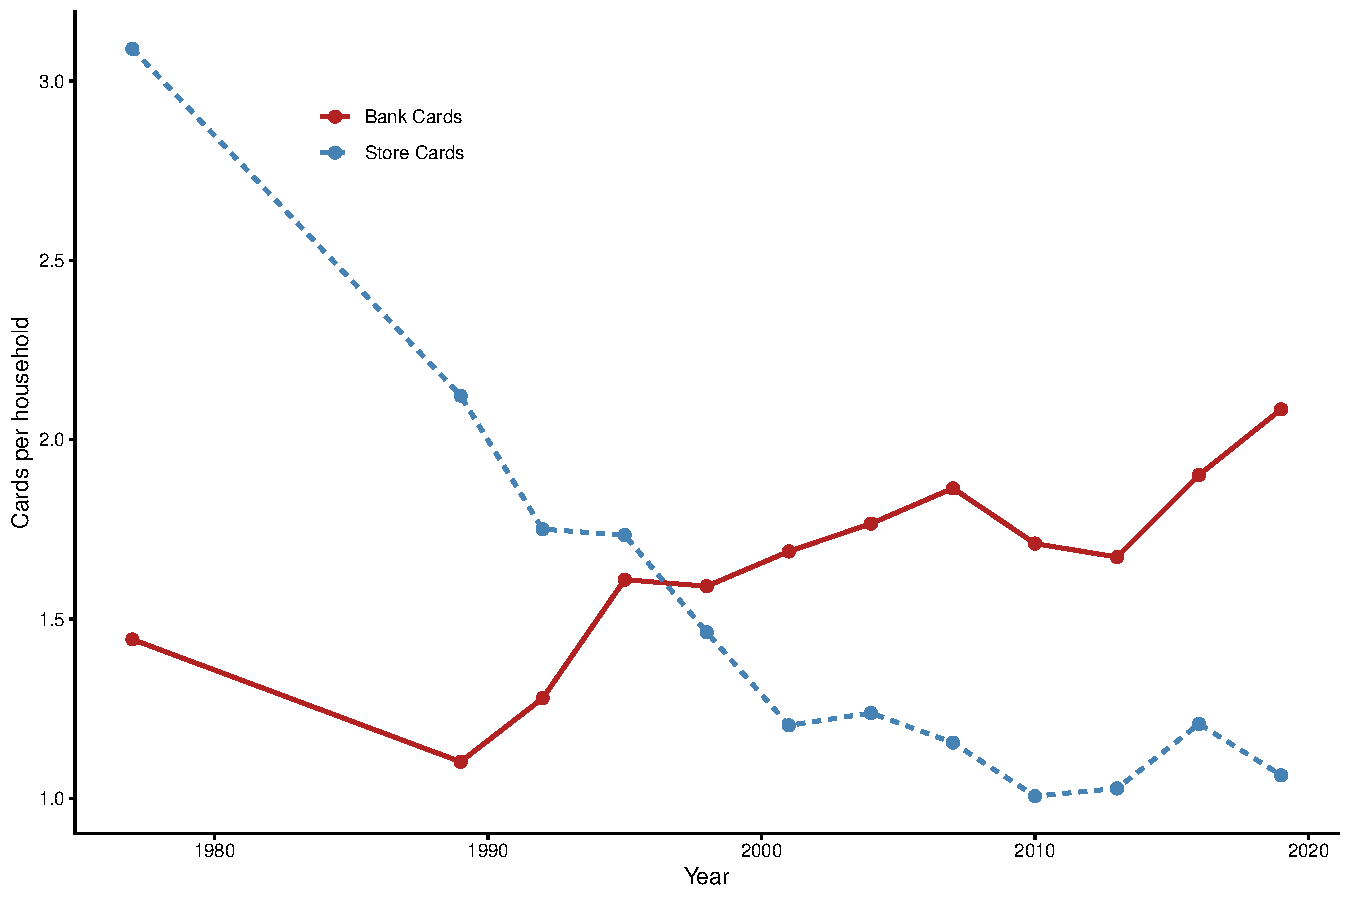
\includegraphics[width=\textwidth]{../Output/Figures/cards_per_household.pdf}
    \tiny Source: SCF
\end{column}
\begin{column}{.32\textwidth}
    \centering
    Household spending \\
    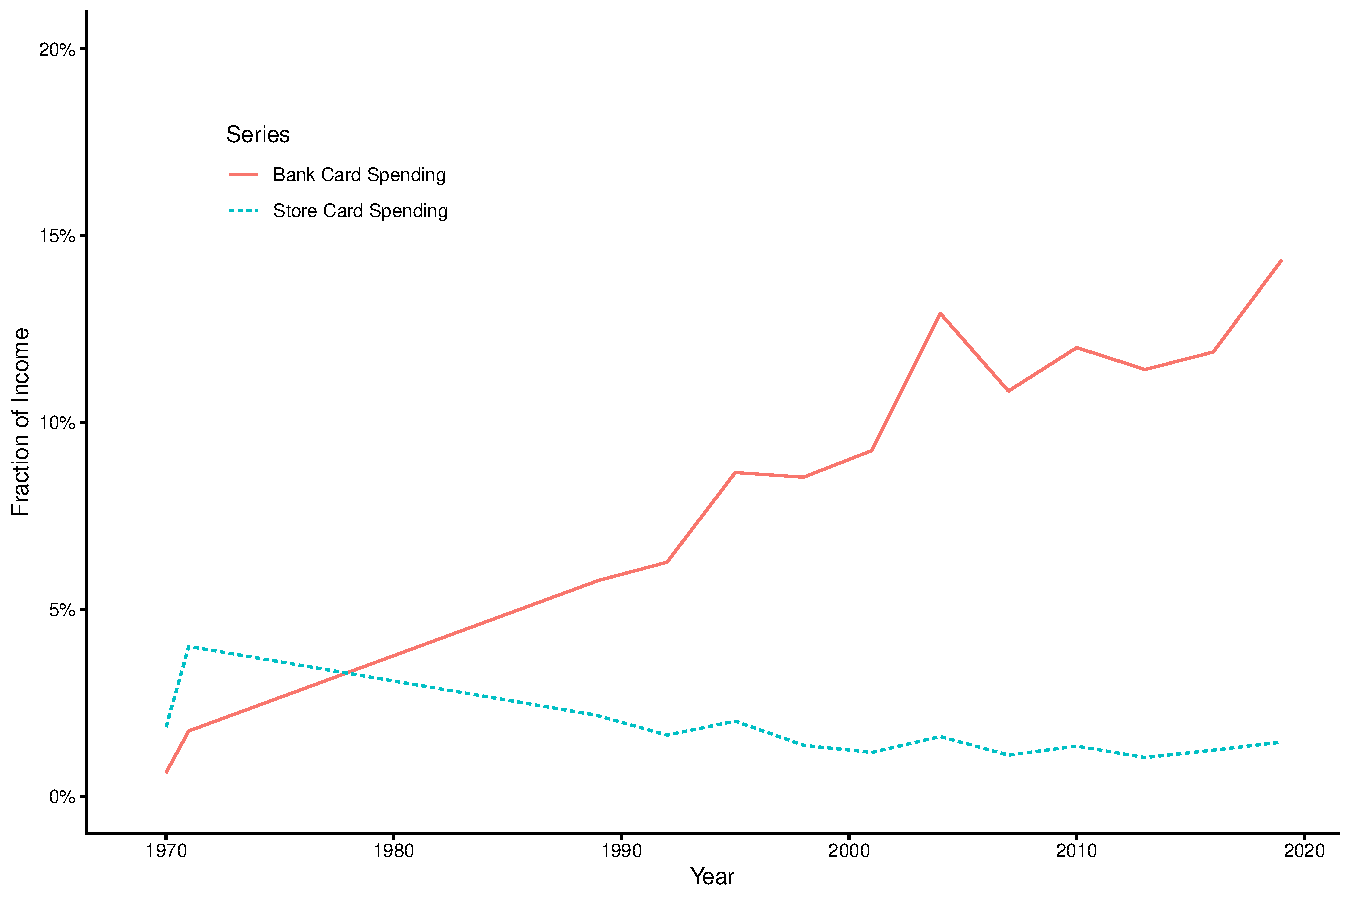
\includegraphics[width=\textwidth]{../Output/Figures/spending_levels.pdf}
    \tiny Source: SCF
\end{column}
\begin{column}{.32\textwidth}
    \centering
    Firm receivables \\
    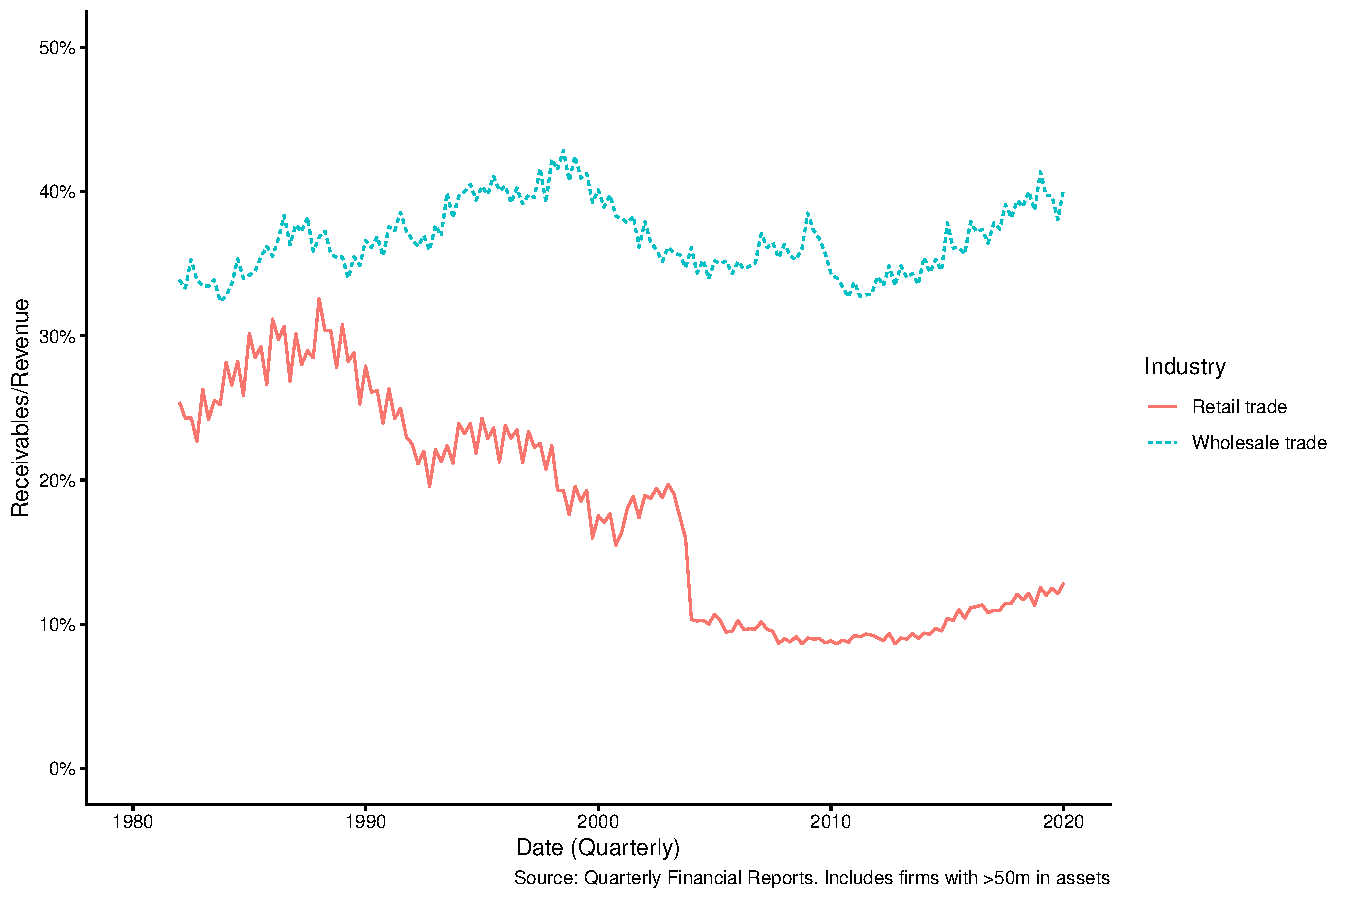
\includegraphics[width=\textwidth]{../Output/Figures/receivables.pdf}
    \tiny Source: US Census QFR (assets $\geq$ \$50M)
\end{column}
\end{columns}
\end{center}

\end{frame}


%% ============================================================
%% SLIDE 5: LABOR COST REDUCTIONS
%% ============================================================
\begin{frame}{Firms Saved on Credit-Related Labor}

Retail firms once spent 4\% of their wage bill on bookkeepers and bill collectors

\begin{center}
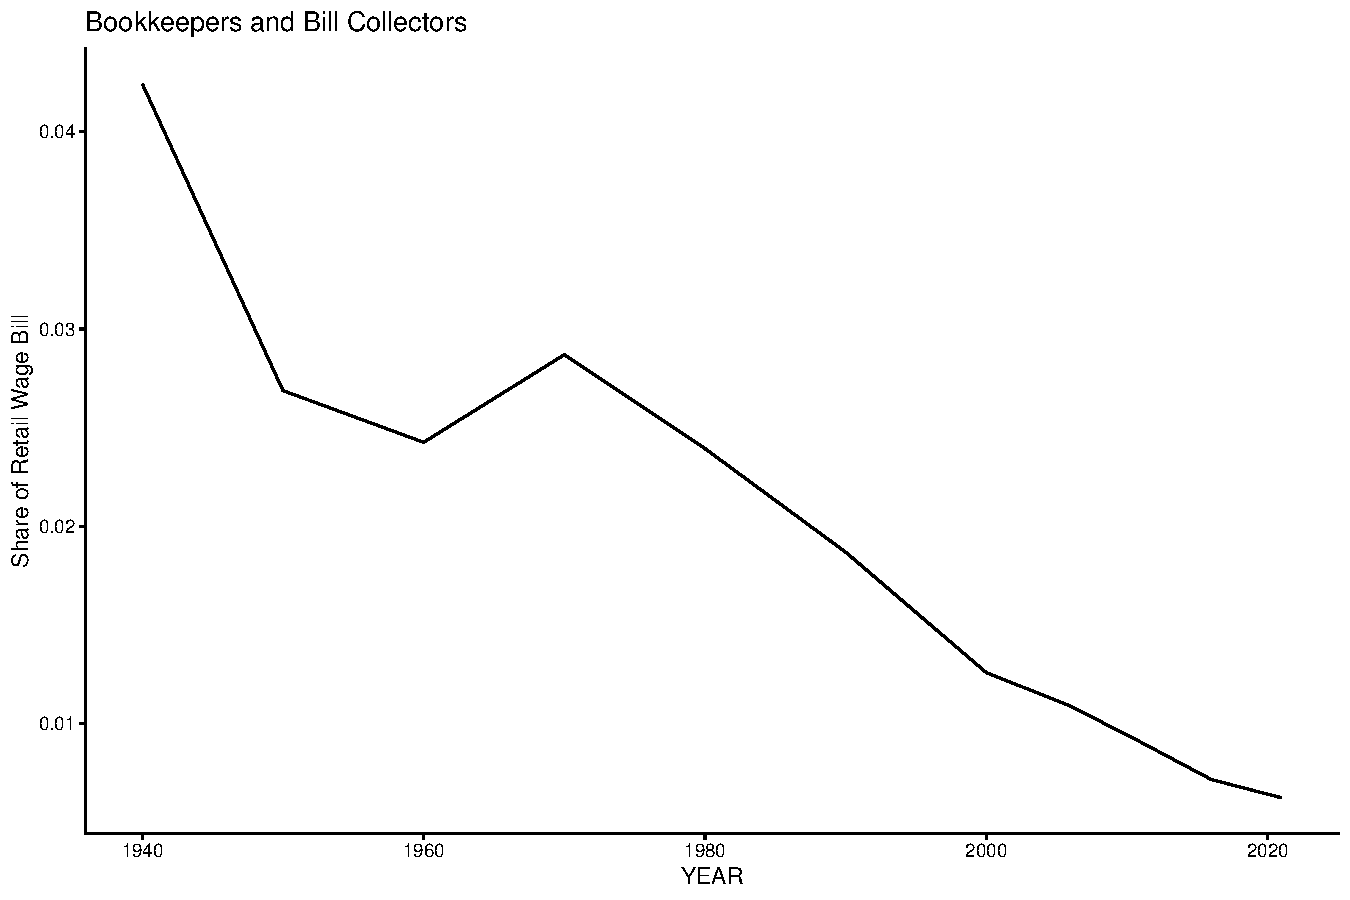
\includegraphics[width=0.55\textwidth]{../Output/Figures/backoffice_retail.pdf}
\end{center}

\small Source: US Census.

\end{frame}


%% ============================================================
%% SLIDE 6: IDENTIFICATION STRATEGY
%% ============================================================
\begin{frame}{Identification: 1978 \emph{Marquette} Decision}

\begin{itemize}
    \item Supreme Court ruled banks can lend across state lines at \emph{home state's} usury rate
    \vfill
    \item States with usury $< 18\%$ in 1977 saw sudden increase in bank card supply from out-of-state banks
    \vfill
    \item 9 ``treated'' states (37M people, 16\% of nation)
    \vfill
    \item Revolving credit regulated separately---no effect on mortgages, business loans
    \vfill
    \item I do \emph{not} use the subsequent endogenous deregulation decisions: only the unexpected Supreme Court shock for identification
\end{itemize}

\end{frame}


%% ============================================================
%% SLIDE 7: VALIDITY OF IDENTIFICATION
%% ============================================================
\begin{frame}{Support for Identification}

\begin{columns}[T]
\begin{column}{.45\textwidth}
    \centering
    No geographic pattern \\[0.3em]
    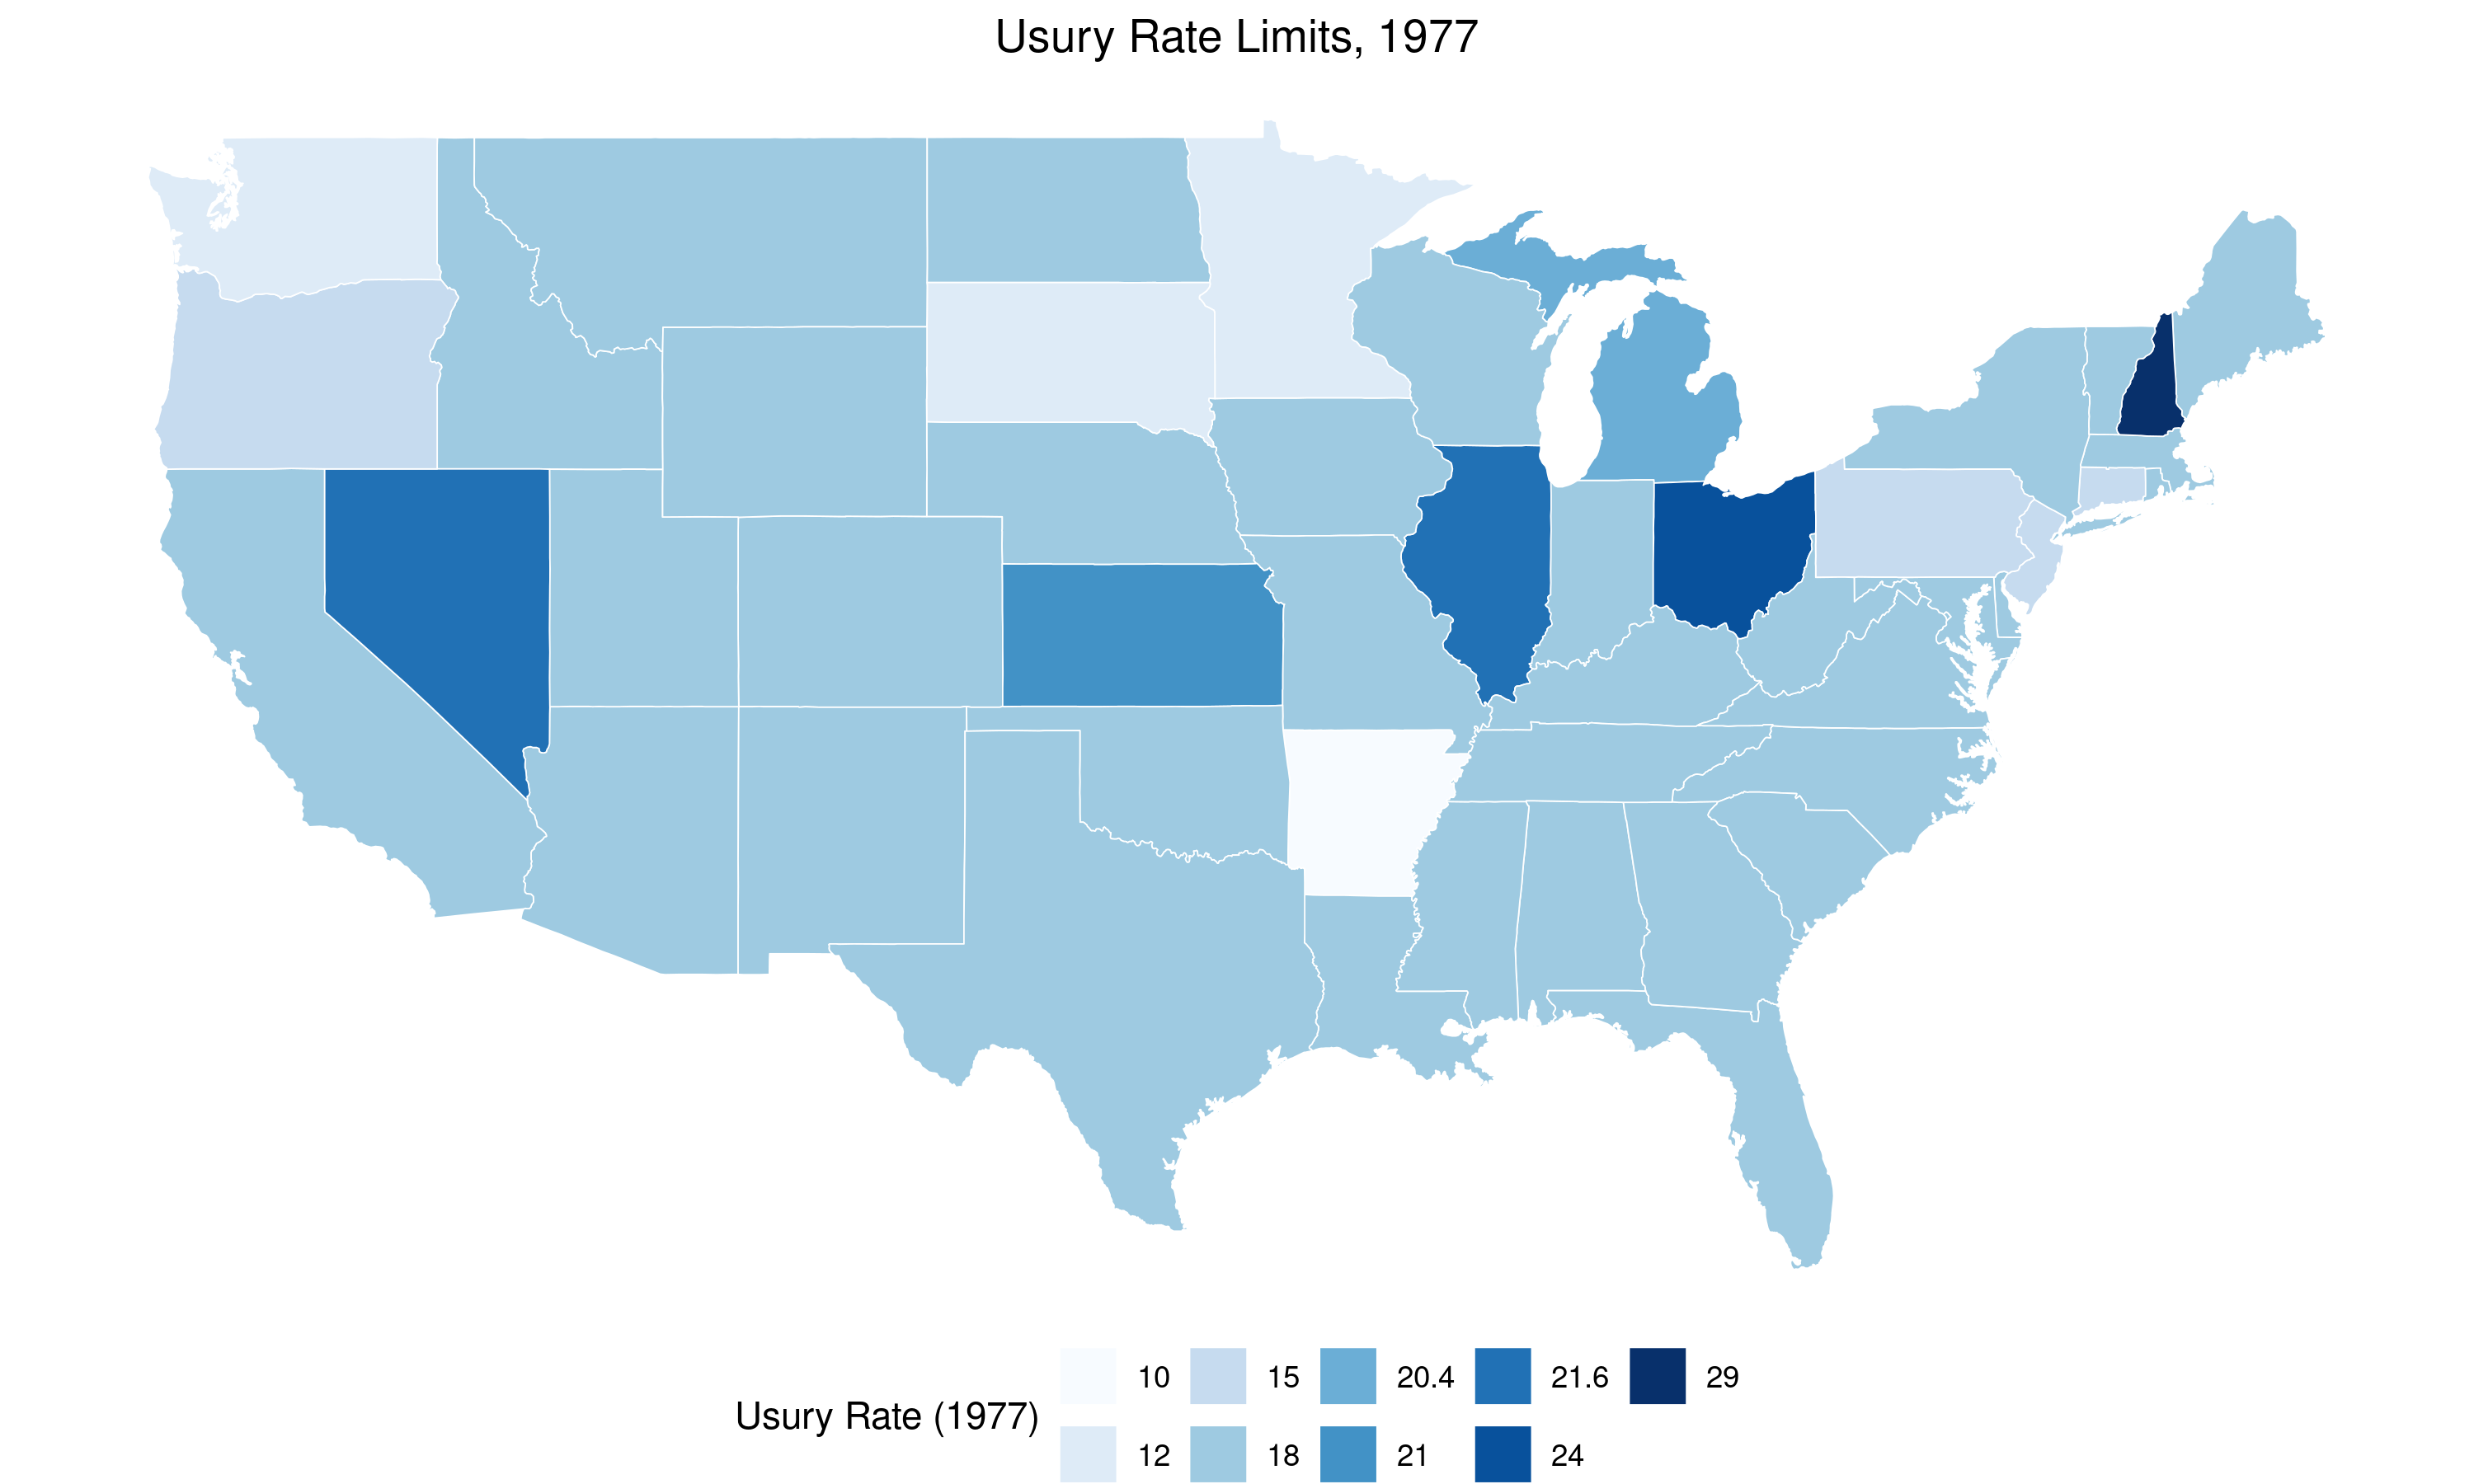
\includegraphics[width=\textwidth]{../Output/Figures/rate_77.png}
    \tiny Source: Cost of Personal Borrowing, 1977
\end{column}
\hfill
\begin{column}{.45\textwidth}
    \centering
    Orthogonal to other deregulation \\[0.3em]
    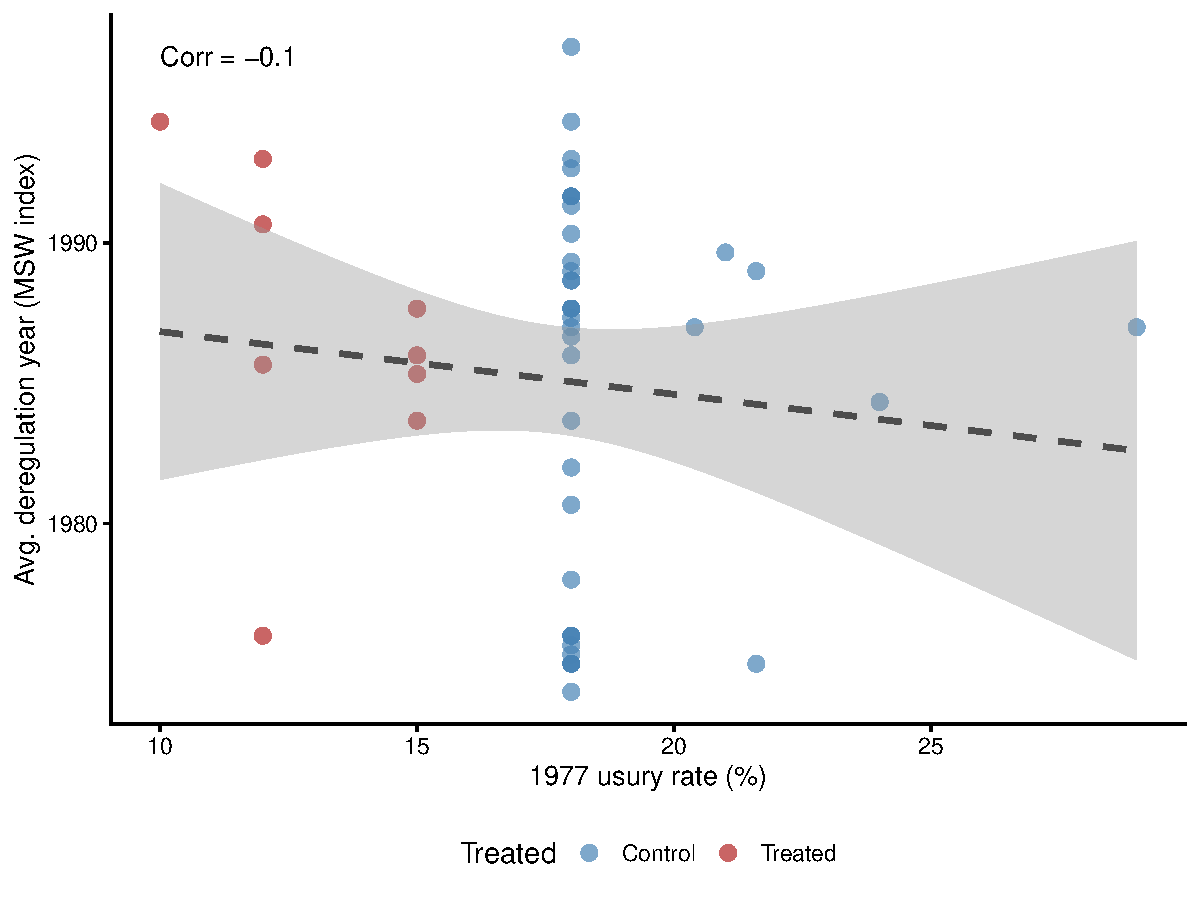
\includegraphics[width=0.9\textwidth]{../Output/Figures/msw_correlation.pdf}
    \tiny Corr $= -0.10$ with Mian-Sufi-Verner deregulation index
\end{column}
\end{columns}

\vfill
\small Treatment balance: no significant differences in wages, employment, GDP, or retail share between treated and control states in 1977

\end{frame}


%% ============================================================
%% SLIDE 8: USURY RATES BINDING
%% ============================================================
\begin{frame}{Usury Limits Were Binding}

\begin{columns}[T]
\begin{column}{.48\textwidth}
\centering
1977: Bunching at limits \\
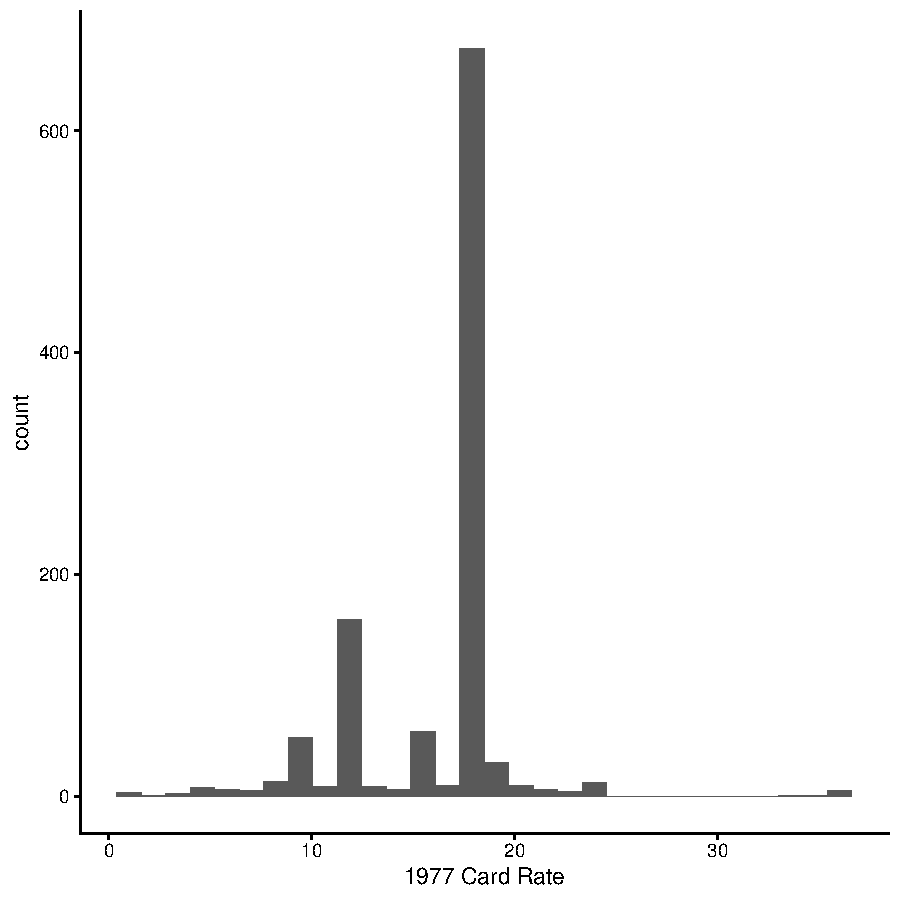
\includegraphics[width=\textwidth]{../Output/Figures/bunching}
\end{column}
\begin{column}{.48\textwidth}
\centering
1983: Limits no longer bind \\
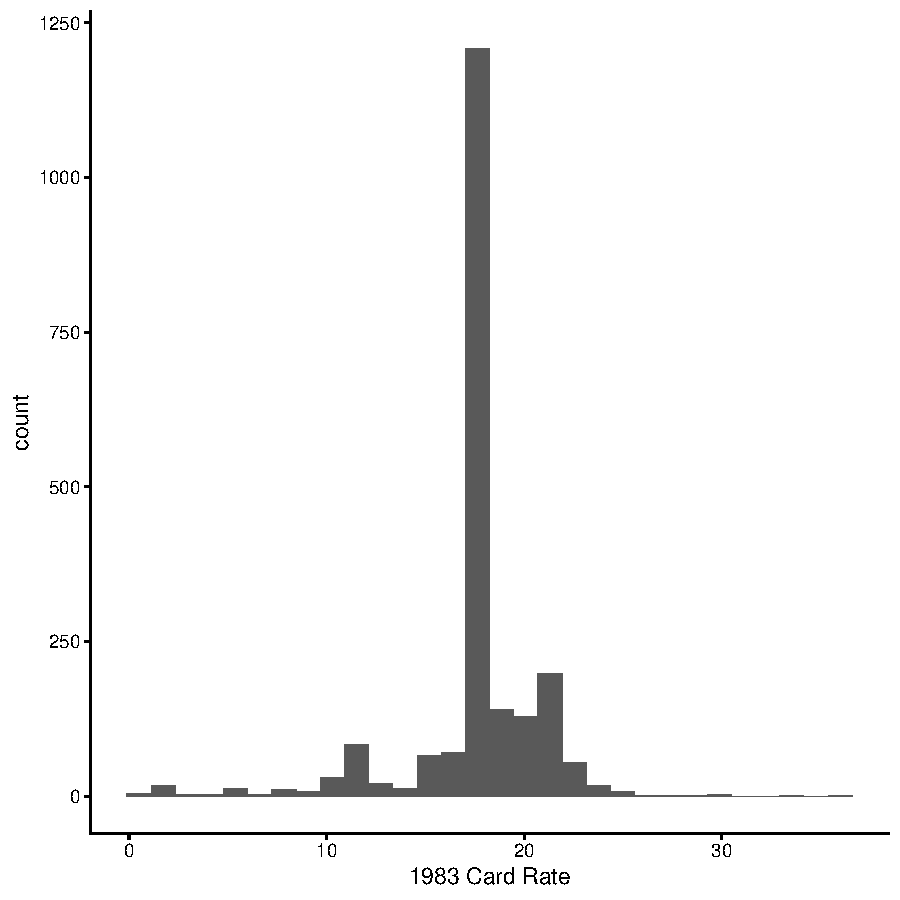
\includegraphics[width=\textwidth]{../Output/Figures/bunching_83}
\end{column}
\end{columns}

\end{frame}


%% ============================================================
%% SLIDE 9: CARD LENDING GROWTH
%% ============================================================
\begin{frame}{Card Lending Grew from Deregulated-State Banks}

\begin{center}
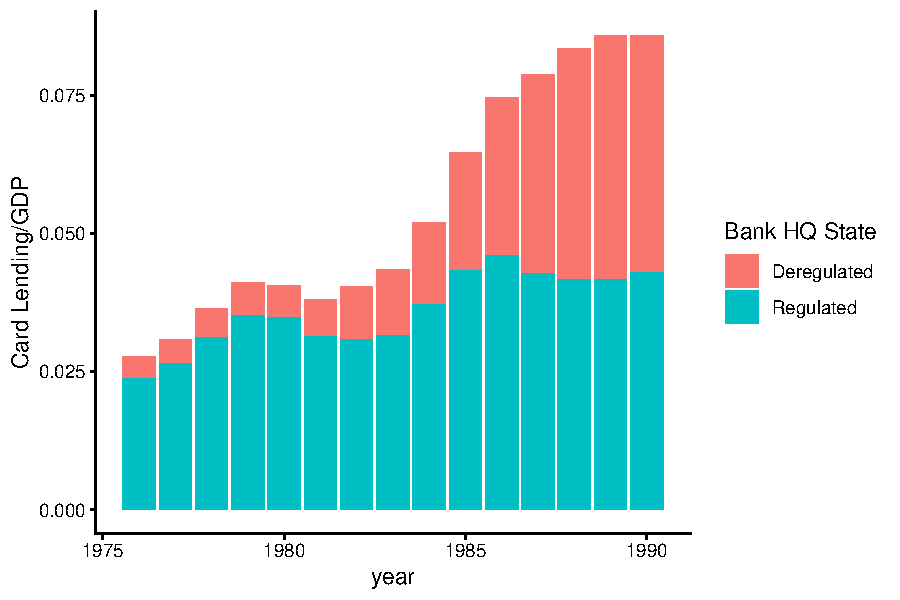
\includegraphics[width=0.65\textwidth]{../Output/Figures/card_growth_stacked.pdf}
\end{center}

\small Card lending / GDP by bank HQ state usury regime. Credit card lending tripled 1976--1990; almost all growth from banks headquartered in deregulated states.

\end{frame}


%% ============================================================
%% SLIDE 10: NEW DATA — YELLOW PAGES
%% ============================================================
\begin{frame}{New Data on Bank Card Acceptance}

\begin{columns}[T]
\begin{column}{.3\textwidth}
\centering
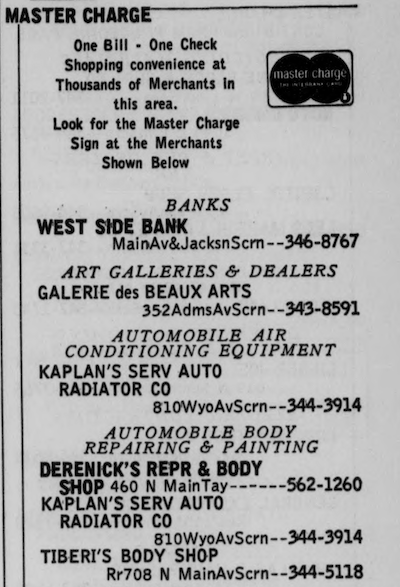
\includegraphics[width=\textwidth]{Static/yellowpages_mc.png}
\end{column}
\begin{column}{.25\textwidth}
\centering
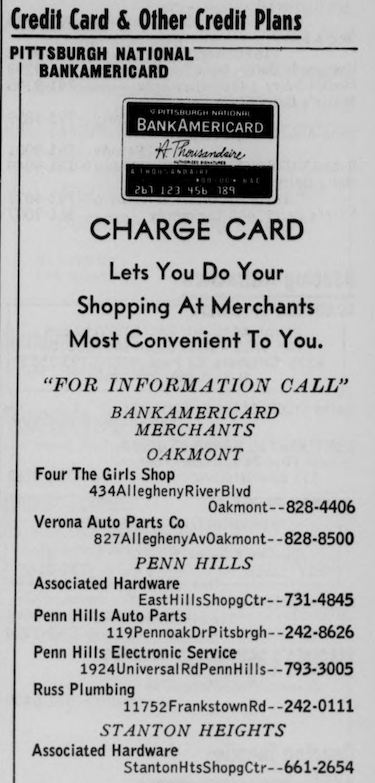
\includegraphics[width=\textwidth]{Static/yellowpages_visa.png}
\end{column}
\begin{column}{.4\textwidth}
\small
\begin{itemize}\setlength\itemsep{0.3em}
    \item U.S.\ Telephone Directory Collection, Library of Congress
    \item 1.97M firm-years screened in Dun \& Bradstreet
    \item 141K covered by phonebooks across 418 municipalities
    \item 510 card-accepting merchant-years manually transcribed and matched to D\&B
    \item Final sample: Compustat firms matched to D\&B sales locations, with sales from D\&B and card acceptance from phonebooks (2,956 firms, 283 markets, 1970--1977)
\end{itemize}
\end{column}
\end{columns}

\end{frame}


%% ============================================================
%% SLIDE 11: COMPUSTAT RESULTS
%% ============================================================
\begin{frame}{Store Lending Fell, Profits Rose}

\begin{columns}[T]
\begin{column}{.55\textwidth}
\centering
Receivables/Revenue fell \\[0.3em]
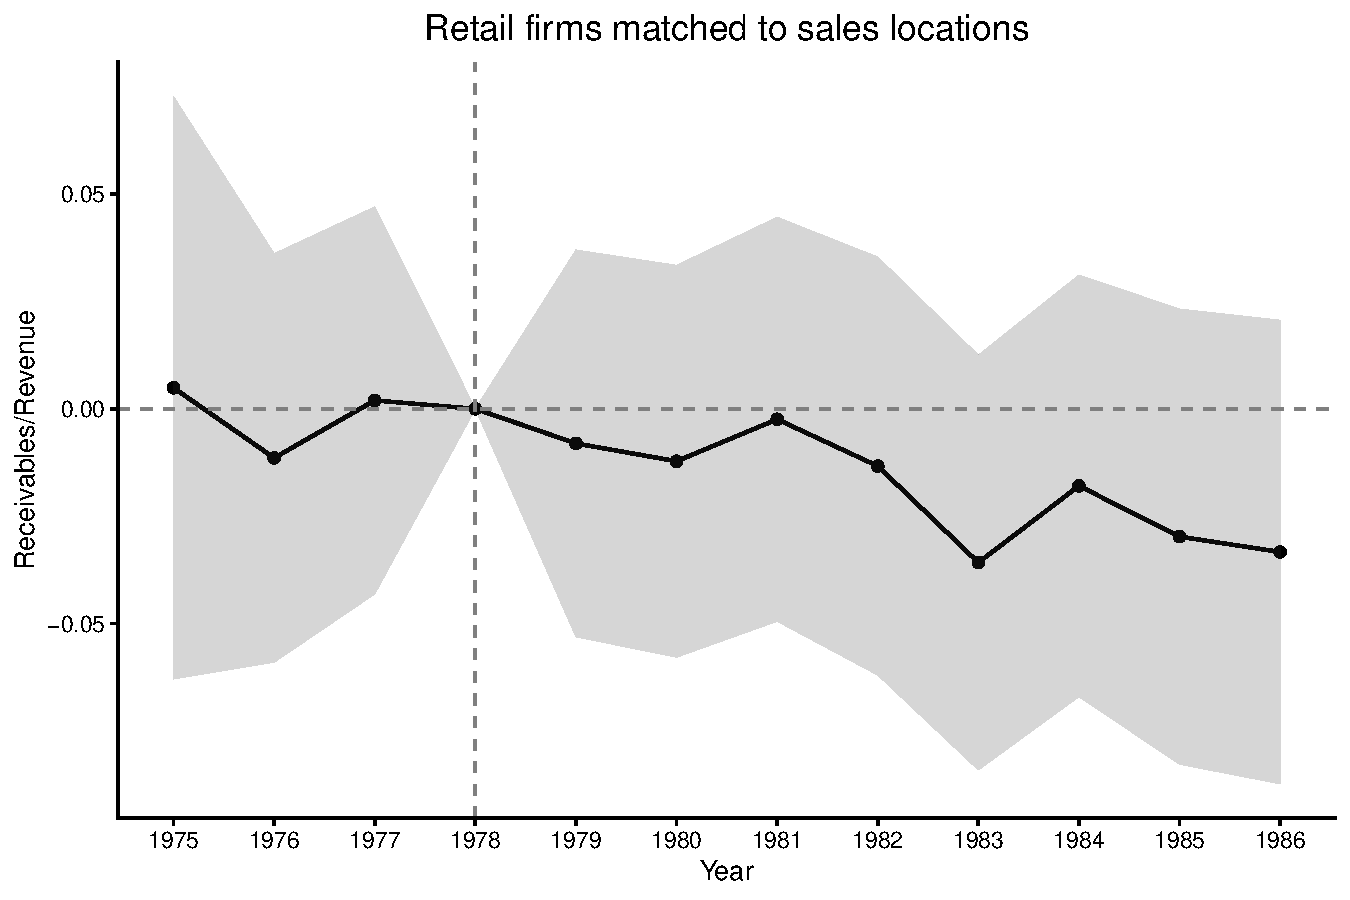
\includegraphics[width=\textwidth]{../Output/Figures/receivables_revenue.pdf}
\tiny 175 retail firms in Compustat
\end{column}
\hfill
\begin{column}{.42\textwidth}
\vspace{1em}
\footnotesize
\resizebox{\columnwidth}{!}{
\begingroup
\centering
\begin{tabular}{lc}
   \tabularnewline \midrule \midrule
   Dependent Variable:    & Net Income / Revenue\\  
   Model:                 & (1)\\  
   \midrule
   \emph{Variables}\\
   Treated $\times$ Post  & 0.0091$^{*}$\\   
                          & (0.0054)\\   
   \midrule
   \emph{Fixed-effects}\\
   Year FE                & Yes\\  
   Firm FE                & Yes\\  
   \midrule
   \emph{Fit statistics}\\
   Observations           & 2,000\\  
   R$^2$                  & 0.21338\\  
   Within R$^2$           & 0.00058\\  
   \midrule \midrule
   \multicolumn{2}{l}{\emph{Clustered (Firm FE) standard-errors in parentheses}}\\
   \multicolumn{2}{l}{\emph{Signif. Codes: ***: 0.01, **: 0.05, *: 0.1}}\\
\end{tabular}
\par\endgroup


}
\vspace{0.5em}
\tiny DV: net income / revenue (post-1978 level shift) \\
At 5\%, we reject that profits fell by more than 15bp
\end{column}
\end{columns}

\end{frame}


%% ============================================================
%% SLIDE 10: NET ENTRY --- TRIPLE DIFF
%% ============================================================
\begin{frame}{Net Entry: Triple-Difference by Industry}

Entrepreneurs also use credit cards to \emph{fund} their businesses. The triple-difference isolates the \emph{payment} channel: clothing retail had the highest card payment intensity, independent of card use by owners as borrowers. Compare to other retail sub-industries:

\begin{columns}[T]
\begin{column}{.32\textwidth}
  \centering
  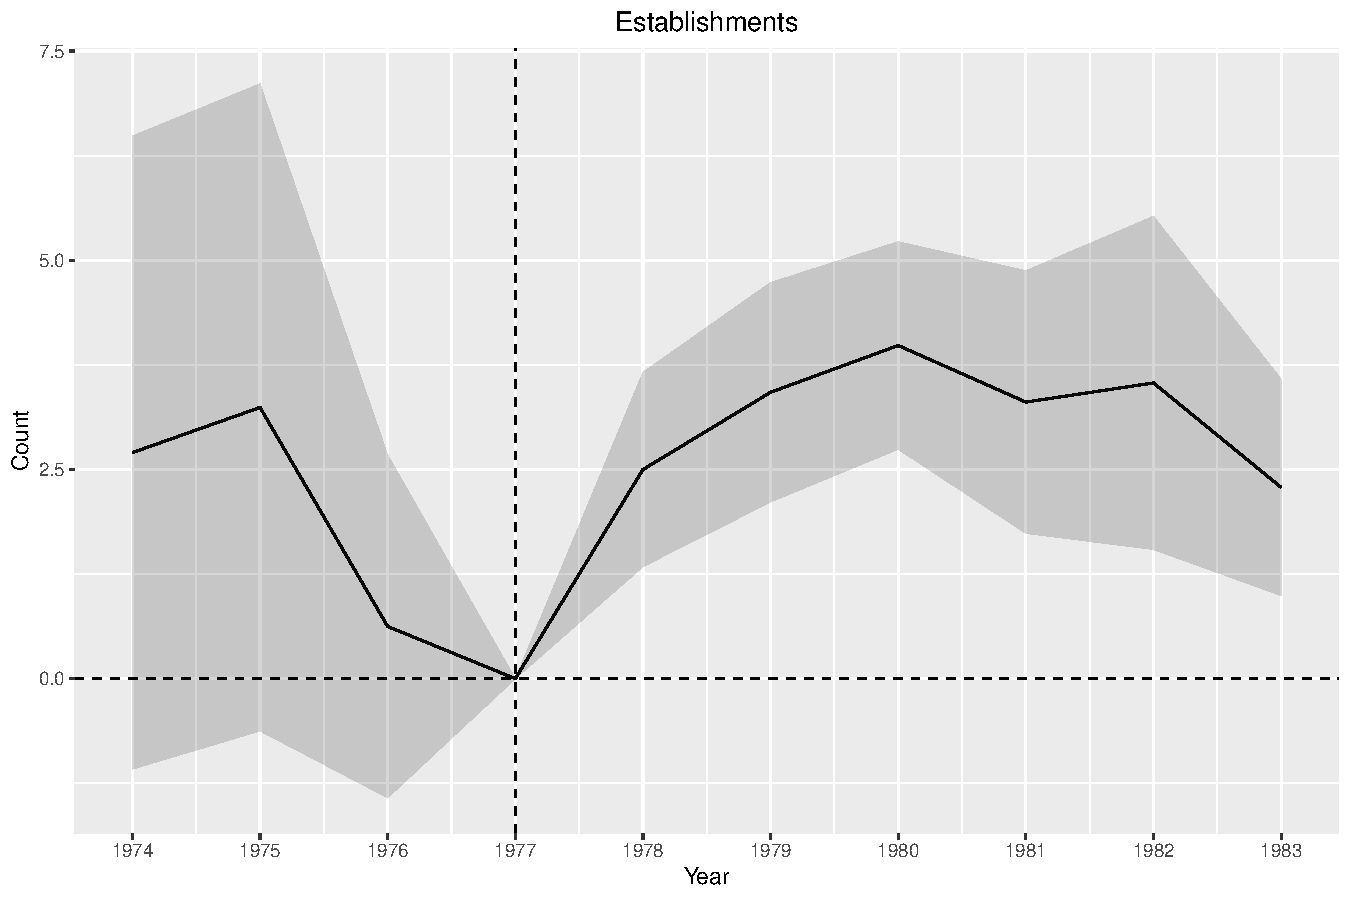
\includegraphics[width=\textwidth]{../Output/Figures/est.pdf}
  \tiny (a) Establishments
\end{column}
\begin{column}{.32\textwidth}
  \centering
  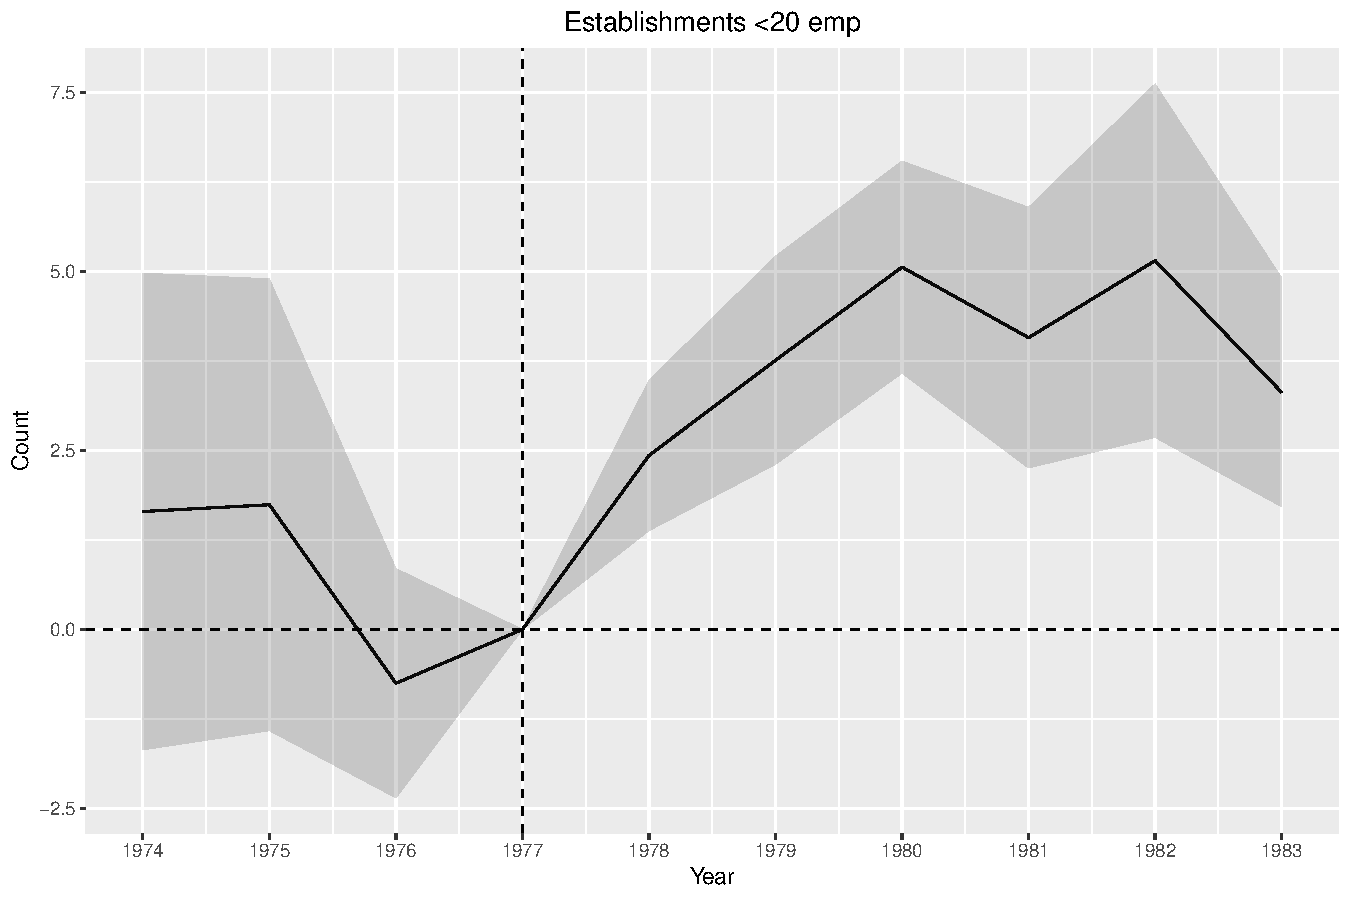
\includegraphics[width=\textwidth]{../Output/Figures/n1_19.pdf}
  \tiny (b) Small establishments
\end{column}
\begin{column}{.32\textwidth}
  \centering
  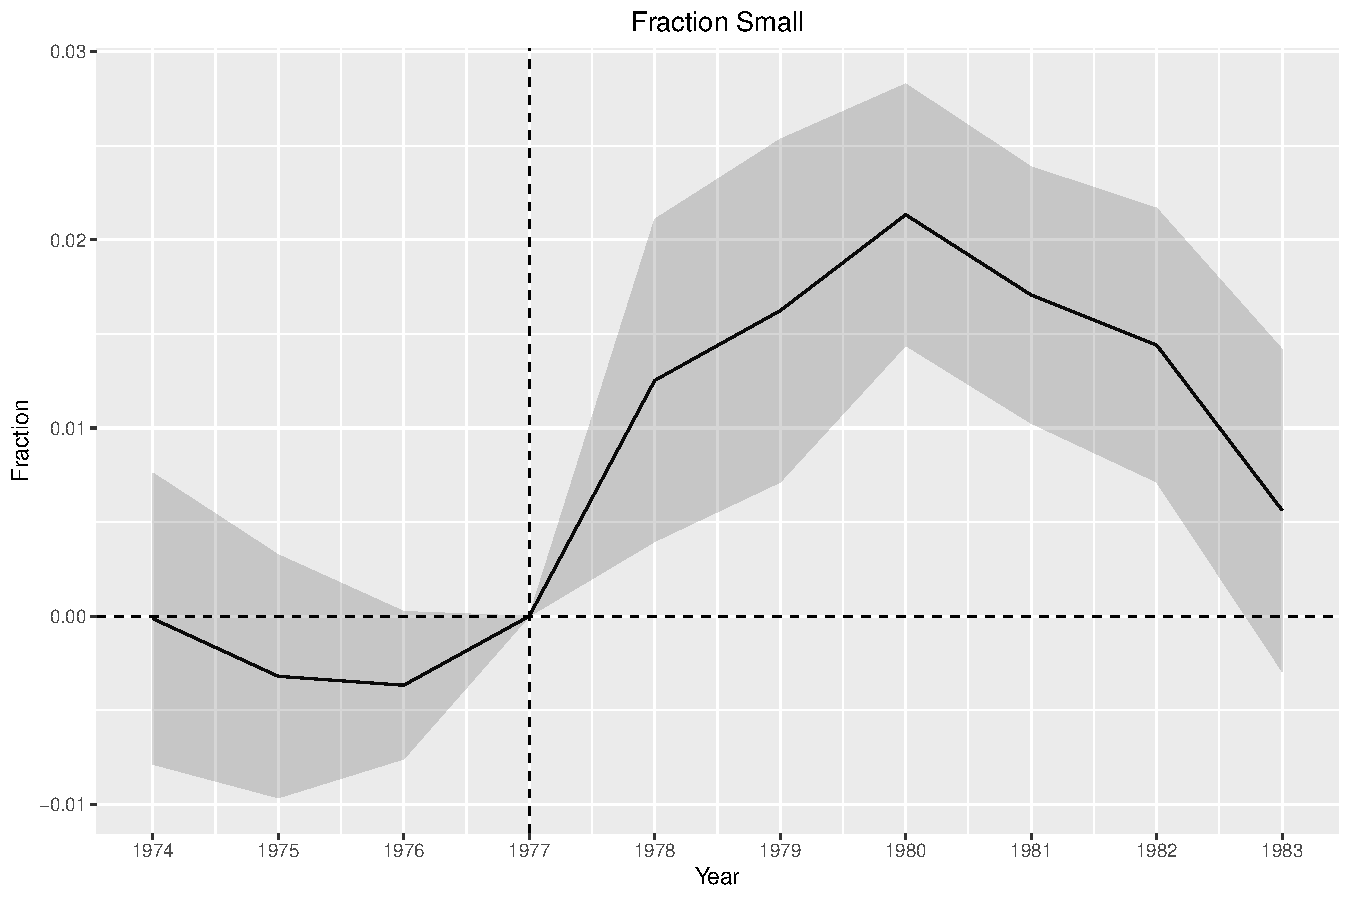
\includegraphics[width=\textwidth]{../Output/Figures/frac_small.pdf}
  \tiny (c) Fraction small
\end{column}
\end{columns}

\vfill

\small 4\% increase in establishments; entrants are disproportionately small.

\end{frame}


%% ============================================================
%% SLIDE 11: WHICH FIRMS ADOPT
%% ============================================================
\begin{frame}{Which Firms Adopt Bank Cards?}

\centering
\scalebox{0.55}{\begingroup
\centering
\begin{tabular}{lcc}
   \tabularnewline \midrule \midrule
   Dependent Variable: & \multicolumn{2}{c}{Card acceptance}\\
   Model:                     & (1)            & (2)\\  
   \midrule
   \emph{Variables}\\
   log(Sales)                 & 0.7112$^{***}$ & 0.7243$^{***}$\\   
                              & (0.1500)       & (0.1505)\\   
   Single-establishment       & 0.6874$^{***}$ & 0.7132$^{***}$\\   
                              & (0.2410)       & (0.2308)\\   
   Firm age                   &                & -0.0075\\   
                              &                & (0.0071)\\   
   \midrule
   \emph{Fixed-effects}\\
   Industry $\times$ City FE  & Yes            & Yes\\  
   \midrule
   \emph{Fit statistics}\\
   Observations               & 1,940          & 1,940\\  
   Squared Correlation        & 0.23179        & 0.23384\\  
   Pseudo R$^2$               & 0.24409        & 0.24501\\  
   BIC                        & 1,522.3        & 1,528.6\\  
   \midrule \midrule
   \multicolumn{3}{l}{\emph{Clustered (industry) standard-errors in parentheses}}\\
   \multicolumn{3}{l}{\emph{Signif. Codes: ***: 0.01, **: 0.05, *: 0.1}}\\
\end{tabular}
\par\endgroup
}

\vfill

\small
\begin{itemize}
    \item Geographically concentrated, high-sales firms adopt first
    \item Consistent with cost reduction (undiversified firms benefit most)
    \item Inconsistent with demand-steering (low-share firms benefit most from stealing business)
\end{itemize}

\end{frame}


%% ============================================================
%% SLIDE 12: STRUCTURAL MODEL (CONDENSED)
%% ============================================================
\begin{frame}{Calibrated Model: Cost Reduction vs.\ Competition}

\small
\textbf{Question}: Does accepting bank cards mainly (a) reduce costs or (b) steal customers?

\vspace{0.3em}
Nested logit: \quad $u_{ij} = \delta_j + \varsigma_{g(j)} + (1-\sigma)\varepsilon_{ij}$, \quad where $\delta_j = \alpha \, p_j + \xi_j$

\begin{itemize}\setlength\itemsep{0.1em}
    \item $\sigma$ = fraction of taste dispersion correlated within card-acceptance groups
    \item $\sigma \to 1$: taste shocks vanish; customers choose only on payment method, not what the store sells
    \item $\sigma = 0$: payment method irrelevant; customers choose on price and idiosyncratic tastes
\end{itemize}

\vspace{0.3em}

\begin{columns}[T]
\begin{column}{.48\textwidth}
\centering
\textbf{Calibrated Parameters}
\begin{tabular}{lc}
\toprule
Parameter & Value \\
\midrule
$\alpha$ (price sensitivity) & $-4$ \\
$\sigma$ (card differentiation) & 0.07 \\
$\zeta$ (cost change) & $-0.07$ \\
\midrule
Implied cost reduction & 2.7\% \\
\bottomrule
\end{tabular}
\end{column}
\begin{column}{.48\textwidth}
\centering
\textbf{Decomposition}
\begin{tabular}{lcc}
\toprule
 & Cost & Markup \\
\midrule
Baseline $\to$ Marquette & $-57$bp & $-9$bp \\
Cost only & $-57$bp & $+12$bp \\
Competition only & 0 & $-21$bp \\
\bottomrule
\end{tabular}
\end{column}
\end{columns}

\vfill
\small $\sigma \approx 0$: cards barely steer customers. Cost reduction dominates; firms \emph{gain} despite slight markup compression.

\end{frame}


%% ============================================================
%% SLIDE 13: INTERNATIONAL CONTEXT
%% ============================================================
\begin{frame}{International Context}

\begin{center}
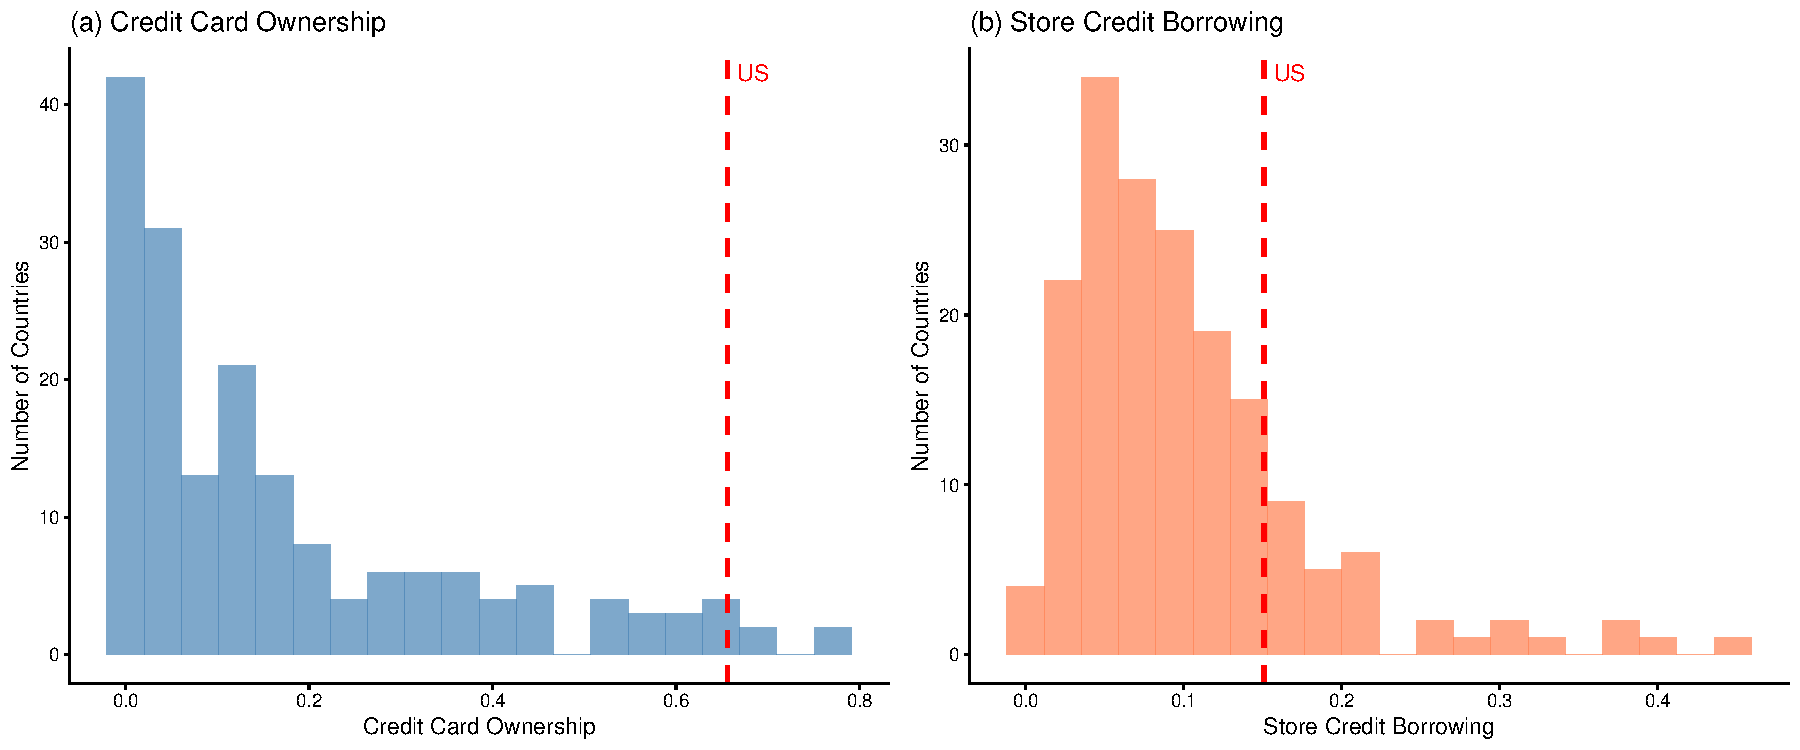
\includegraphics[width=0.9\textwidth]{../Output/Figures/international_histograms.pdf}
\end{center}

\small Many developing countries still rely heavily on store credit. The U.S.\ historical experience suggests that enabling bank-provided consumer credit can reduce costs for small merchants.

\end{frame}


%% ============================================================
%% SLIDE 14: CONCLUSION + POLICY
%% ============================================================
\begin{frame}{Conclusion and Policy Implications}

\textbf{Summary of findings:}
\begin{itemize}
    \item Bank cards displaced store credit, reducing merchants' labor and risk costs
    \item Net effect on retail industry: $+$4\% entry, $+$2\% profits, better recession survival
    \item Cost reduction ($\sim$3\%) dominates markup compression (9bp)
\end{itemize}

\vfill

\textbf{Implications for interchange fee regulation:}
\begin{itemize}
    \item Interchange fees replaced even higher in-house credit costs
    \item Small merchants benefit most from outsourcing credit to banks
    \item Capping fees may force merchants back toward costly in-house credit
    \item Historical evidence: the \emph{net} effect of card networks on merchants was positive
\end{itemize}

\end{frame}


%% ============================================================
%% BACKUP SLIDES
%% ============================================================
\appendix

\begin{frame}[noframenumbering]{Backup: Sensitivity to $\alpha$}
\centering
\begin{tabular}[t]{rrrr}
\toprule
$\alpha$ & $\sigma$ & $\zeta$ & Cost reduction\\
\midrule
-2.000 & 0.0669 & -0.1882 & -0.0697\\
-3.000 & 0.0696 & -0.1075 & -0.0398\\
-4.000 & 0.0711 & -0.0740 & -0.0274\\
-5.000 & 0.0722 & -0.0561 & -0.0207\\
-6.000 & 0.0725 & -0.0276 & -0.0102\\
\addlinespace
-0.258 & 0.0526 & -2.3224 & -0.8593\\
\bottomrule
\end{tabular}


\small Cost reduction ranges from 1\% ($\alpha = -6$) to 7\% ($\alpha = -2$). $\sigma$ is stable across specifications.
\end{frame}

\begin{frame}[noframenumbering]{Backup: Card Acceptance by Industry}
\begin{columns}[T]
\begin{column}{.45\textwidth}
\tiny
\begin{tabular}[t]{llrr}
\toprule
industry & acceptance & n & firms\_accepting\\
\midrule
Clothing & 1.5\% & 4513 & 67\\
Furnishing & 0.7\% & 4686 & 34\\
Misc. & 0.6\% & 11982 & 68\\
Auto & 0.5\% & 10154 & 46\\
Department Stores & 0.3\% & 2332 & 7\\
\addlinespace
Hardware & 0.3\% & 3112 & 9\\
Restaurants & 0.1\% & 12794 & 17\\
Food & 0.0\% & 8247 & 2\\
\bottomrule
\end{tabular}

\end{column}
\hfill
\begin{column}{.45\textwidth}
\tiny
\begin{tabular}[t]{lll}
\toprule
Card use & Store cards & Bank cards\\
\midrule
Clothing & 84\% & 54\%\\
Appliances & 15\% & 9\%\\
Misc. & 15\% & 38\%\\
Household goods & 14\% & 5\%\\
Recreation items & 8\% & 5\%\\
\addlinespace
Hardware & 5\% & 5\%\\
Furniture & 4\% & 10\%\\
Travel & 0\% & 27\%\\
\bottomrule
\end{tabular}

\end{column}
\end{columns}
\end{frame}

\begin{frame}[noframenumbering]{Backup: Recession Survival}
\tiny
\begingroup
\centering
\begin{tabular}{lcccc}
   \tabularnewline \midrule \midrule
   Dependent Variable: & \multicolumn{4}{c}{Exit rate}\\
   Model:                                              & (1)             & (2)             & (3)             & (4)\\  
   \midrule
   \emph{Variables}\\
   Mean log(Sales)                                     & -0.0092$^{***}$ & -0.0127$^{***}$ & -0.0107$^{***}$ & -0.0155$^{***}$\\   
                                                       & (0.0004)        & (0.0008)        & (0.0005)        & (0.0008)\\   
   Treated $\times$ Single-estab.                      & -0.0006         & -0.0016         & -0.0020         & -0.0041$^{**}$\\   
                                                       & (0.0027)        & (0.0026)        & (0.0015)        & (0.0019)\\   
   Single-estab. $\times$ Recession                    & 0.0459$^{***}$  & 0.0514$^{***}$  & 0.0305$^{***}$  & 0.0159$^{***}$\\   
                                                       & (0.0039)        & (0.0046)        & (0.0033)        & (0.0022)\\   
   Treated $\times$ Recession $\times$ Single-estab.   & -0.0159$^{*}$   & -0.0204$^{**}$  & 0.0003          & 0.0072\\   
                                                       & (0.0081)        & (0.0099)        & (0.0113)        & (0.0084)\\   
   \midrule
   \emph{Fixed-effects}\\
   State $\times$ Industry $\times$ Year FE            & Yes             & Yes             & Yes             & Yes\\  
   \midrule
   \emph{Fit statistics}\\
   Observations                                        & 73,036          & 27,252          & 73,036          & 27,252\\  
   R$^2$                                               & 0.99726         & 0.99720         & 0.99718         & 0.99704\\  
   Within R$^2$                                        & 0.11503         & 0.17114         & 0.08924         & 0.12386\\  
   \midrule \midrule
   \multicolumn{5}{l}{\emph{Clustered (STATE) standard-errors in parentheses}}\\
   \multicolumn{5}{l}{\emph{Signif. Codes: ***: 0.01, **: 0.05, *: 0.1}}\\
\end{tabular}
\par\endgroup

\end{frame}

\begin{frame}[noframenumbering]{Backup: DiD with Controls}
\begin{columns}[T]
\begin{column}{.48\textwidth}
\centering
Baseline \\
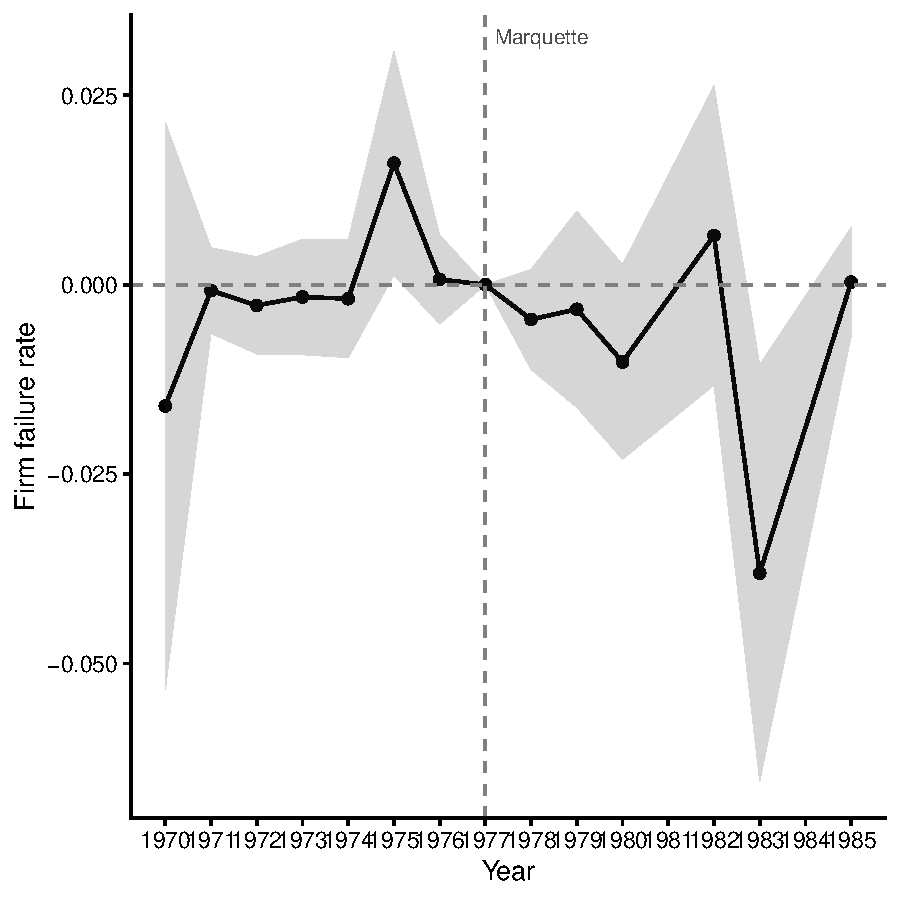
\includegraphics[width=\textwidth]{../Output/Figures/difdif_exit_all.pdf}
\end{column}
\begin{column}{.48\textwidth}
\centering
With state controls \\
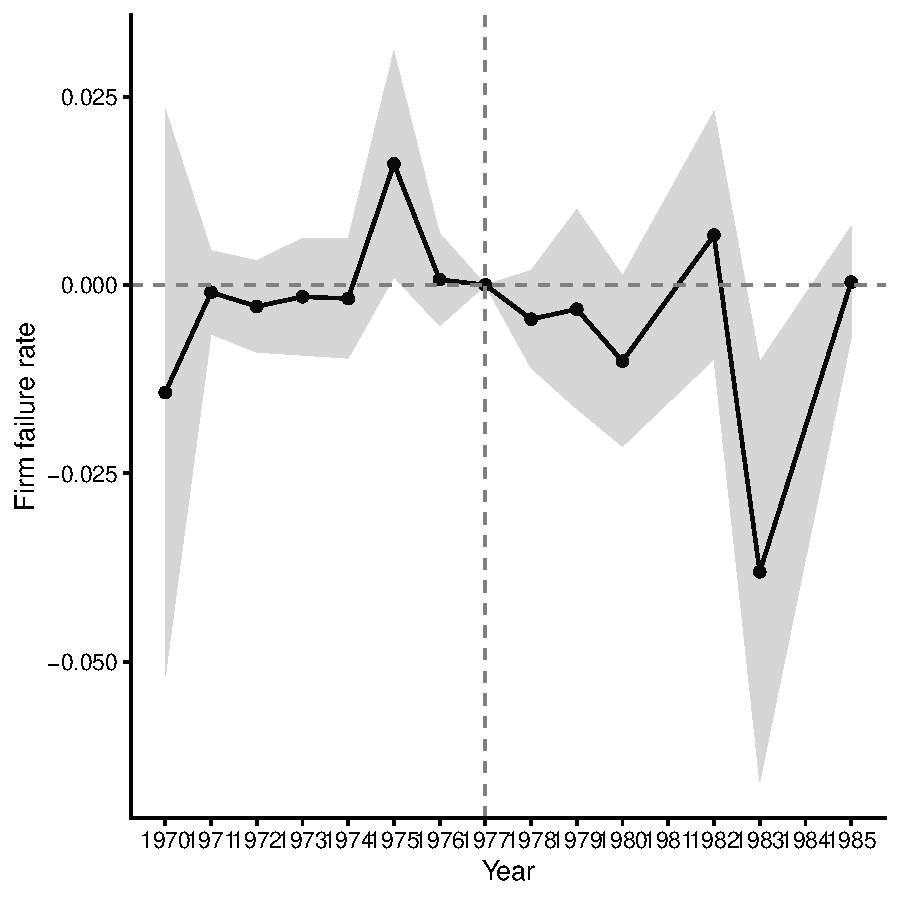
\includegraphics[width=\textwidth]{../Output/Figures/difdif_exit_controls.pdf}
\end{column}
\end{columns}
\small Results robust to controlling for baseline state wages and employment interacted with year FE.
\end{frame}

\end{document}
